\section{Het project}
\label{project}

\index{Project}

\subsection{Informatie vooraf}

\index{Project!informatie}

Delem besturingen communiceren met de zogenaamde \index{CAN}CAN-bus naar modulen. Een \index{Module}module kan bijvoorbeeld een motor aansturen, die er bijvoorbeeld voor zorgt dat de persbalk naar een bepaalde positie gaat.

\subsection{Organisatie}
\label{organisatie}

De \index{Opdrachtgever}opdrachtgever van het project is de firma Delem, die als stagebegeleider de heer M. Scholte heeft aangewezen.

De \index{Opdrachtnemer}opdrachtnemer is de heer R. Springer, student van Fontys Hogescholen te Eindhoven. De begeleidende docent is de heer H. van Heumen.

\subsection{Probleemstelling}

\index{Project!probleemstelling}
\label{probleemstelling}

Op het moment is er geen manier waarop modulen specifiek getest kunnen worden. Om nu een module te testen wordt er soms een compleet systeem gebouwd met besturing en motoren.

Aangezien dit niet praktisch is, hebben engineers zelf oplossingen bedacht om toch zoveel mogelijk lokaal te kunnen testen. Hierbij werd vooral de scripttaal \index{Perl}Perl\footnote{www.perl.com} gebruikt, samen met een hele hoop tooltjes.

\subsection{Resultaat}
\index{Project!resultaat}

De bedoeling is een programma te ontwikkelen dat modulen kan testen. Aangezien er nog onduidelijk is wat er het beste getest kan worden en welke CAN PC hardware het beste gebruikt kan worden, zal er eerst een \index{Analyse}analyse uitgevoerd worden om te kijken welke hardware het beste voldoet.

De functionaliteit die er absoluut in moet zitten, is het leesbaar weergeven van berichten op de CAN bus, alsmede de mogelijkheid om zelf berichten naar modulen te kunnen sturen. Dit kan niet met conventionele programma's, aangezien Delem zelf berichten toegevoegd heeft die niet in de CAN specificatie staan. Extra functionaliteit zal na de analyse en in de loop van het project toegevoegd worden.

\subsection{Randvoorwaarden}

De \index{Randvoorwaarden} randvoorwaarden van dit project zijn als volgt:

\begin{itemize}
\item Alle toegezegde middelen blijven beschikbaar tot het eind van de stageperiode.
\item Belanghebbenden van het project maken genoeg tijd beschikbaar voor ondersteuning van de stagiair.
\end{itemize}

\subsection{Risico's}
\index{Risico's}

Zoals bij elke stageopdracht is er het risico dat er niet genoeg kennis bij de stagiair aanwezig is, wat als resultaat heeft dat het project niet op tijd af komt. Aan de hand van de ervaring van de bedrijfsbegeleider en de kennis van de aanwezige ICT-ers bij het bedrijf en de stagiair zelf is de kans dat dit gebeurt klein.

\subsection{Fasering}

\label{fasering}
\index{Fasering}

Bij Delem wordt de doorlooptijd van projecten in zogenaamde \index{Milestones}\emph{milestones} verdeeld. Milestones worden weer onderverdeeld in zogenaamde \index{Increments}\emph{increments}, een periode van 2 weken. Hieronder is een overzicht te vinden van de milestones, inclusief hun rol met betrekking tot dit project:

\newpage
\subsubsection{Overzicht}

\label{faseringoverzicht}
\index{Fasering!overzicht}
\begin{figure}[h]
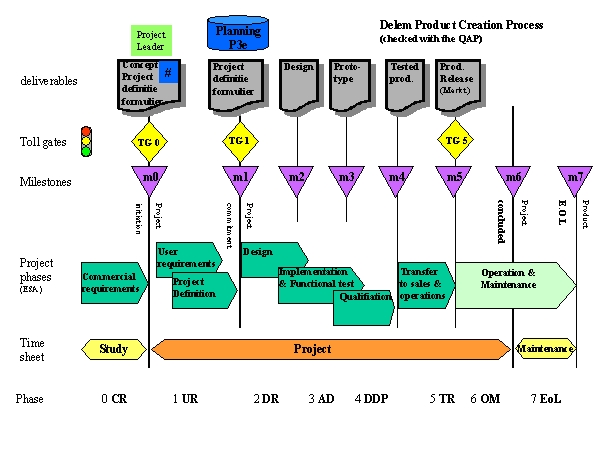
\includegraphics[width=\textwidth]{proces.jpg}
\end{figure}

\subsubsection{Toelichting}
\index{Fasering!toelichting}

Hieronder volgt een toelichting van de fasering, zoals die in het plaatje hierboven te zien is:

\begin{itemize}
\item Milestone 0: Studie\\
Het doel hier is het project te defini\"eren. De uitkomst hiervan is normaal gesproken een commerci\"ele beschrijving, zoals wat er nu in \index{SAIS}SAIS\footnote{Fontys' Stage- en Afstudeer Informatie Systeem, zie http://intranet.hi.fontys.nl/sais} te vinden is. Dit wordt een CRS\footnote{Commercial Requirements Specification} genoemd.
\item Milestone 1: Voorbereiding\\
Tijdens deze fase wordt het product formeel voorbereid. Hierbij worden vooral zaken geanalyseerd. Het hoofdstuk planning op bladzijde \pageref{planning} in dit Plan van Aanpak wordt uitgebreid aan de hand van de bevindingen hiervan. Het directe resultaat is het Plan van Aanpak. Dit wordt een \index{URD}URD\footnote{User Requirements Document} genoemd.
\item Milestone 2: Ontwerp\\
In deze fase wordt het product echt ontworpen. Als het een hardwareproduct is worden de schema's ontwikkeld, bij softwareproducten worden hier bijvoorbeeld de \index{UML}UML\footnote{Universal Modelling Language} schema's getekend.
\item Milestone 3: Implementatie en testen\\
Nu wordt het product daadwerkelijk gemaakt. De bedoeling is dat aan het eind van deze milestone een prototype van het product af is.

Het product wordt tijdens het implementeren ook getest door de ontwikkelaars zelf. Dit resulteert in CR's en PR's, hier zal later op worden ingegaan.
\item Milestone 4: Product test release\\
Hier wordt het product vrijgegeven voor interne release, waar het ook uitgebreid getest gaat worden door de testafdeling. Dit resulteert in nog meer CR's en PR's.
\end{itemize}

Aangezien dit een product voor intern gebruik is, zijn milestone 5: Markt release, milestone 6: Project sluiting en milestone 7: onderhoud weggelaten. De uiteindelijke planning is te vinden op bladzijde \pageref{planning}.

Op de volgende pagina is een overzicht te zien van de projectplanning zoals deze bij Delem gehanteerd wordt:

\subsection{Hulpprogramma's}

\index{Hulpprogramma's}

Er wordt bij Delem gebruikt gemaakt van een drietal programma's, waarmee de bronnen in een project en de status ervan goed bewaakt kunnen worden. Deze programma's zijn:

\begin{itemize}
\index{Primavera!Project Manager}
\item Primavera Project Manager\\
Met dit programma kunnen alle activiteiten omtrent een project ingepland worden. Via \index{Primavera!Progress Reporter}Primavera Progress Reporter kunnen mensen die aan het project werken uren boeken op deze activiteiten. Zo is meteen te zien hoeveel uur ergens voor ingepland werd en hoeveel tijd er daadwerkelijk aan besteed is.
\index{PVCS!Tracker}
\item PVCS Tracker\\
Dit programma slaat de CR's en PR's op in een database, waarop gezocht kan worden. Elke CR en PR heeft een eigenaar, die verantwoordelijk is voor de request. Opmerkingen en dergelijke kunnen bij de CR en PR gevoegd worden, zodat er altijd een goed overzicht is wat de status en geschiedenis van de request is.
\index{PVCS!Version Manager}
\item PVCS Version Manager\\
Dit programma is vergelijkbaar met CVS\footnote{Concurrent Version System, zie www.cvs.org} of diens voorganger RCS\footnote{Revision Control System}. Alle projectbestanden worden hiermee onder versiebeheer geplaatst. Dit zorgt ervoor dat alle veranderingen tot de projectbestanden, of dat nu broncode, documentatie of wat dan ook is, altijd gearchiveerd word.
\end{itemize}

\subsubsection{CR's en PR's}

\index{CR}
\index{PR}
\label{PR}
\label{CR}

Zoals in de vorige paragraaf al naar voren kwam, zijn PR\footnote{Problem Report}'s en CR\footnote{Change Request}'s erg belangrijk. Deze twee zaken kunnen worden gecr\"eerd en opgezocht worden met behulp van de PVCS Tracker.

Het doel hiervan is een duidelijk overzicht te hebben van de taken die voor het project uitgevoerd moeten worden. Verder kan er met behulp van de Progress Reporter aangegeven worden hoeveel tijd er daadwerkelijk gespendeerd is aan een taak, zodat er meteen een duidelijk overzicht is.

\subsubsection{Change Control Board}
\index{CCB}
\label{CCB}
CR's en PR's worden beheerd door middel van een CCB\footnote{Change Control Board}. Als een CR/PR is ingeschoten, dan besluit normaal gesproken het CCB (dit is normaal gesproken een team van de projectleider, projectleden en sales/management personen) of die CR/PR wel of niet gehonoreerd wordt.

\subsection{Analyses}

De volgende analyses zullen worden uitgevoerd:

\begin{itemize}
\item \index{Analyse!hardware}Hardware analyse \\
Het doel van deze analyse is om uit te zoeken wat de beste hardware is om met de modulen te communiceren.
\item \index{Analyse!functionaliteit}Functionaliteit analyse \\
Deze analyse concentreert zich op de functionaliteit die het programma moet krijgen. Om dit te doen zullen de mensen die veel met DM modulen te maken hebben, naar hun mening hierover gevraagd worden. Aan de hand hiervan zal er samen met de bedrijfsbegeleider een overzicht gemaakt worden van functionaliteit die erin moet zitten, functionaliteit die gewenst is en functionaliteit die niet noodzakelijk is.
\end{itemize}
